\chapter{INTRODUCTION}
\label{ch1}
This introduction chapter summarizes the main aerodynamic features of the airplane and
the cost estimate to construct it.

\section{MISSION REQUIREMENTS}
\label{s:ch1_intro}
The objective of this airplane design is to build an aircraft capable of carrying
a payload much greater than its structural weight. The mission profile includes
take-off, a 360 degree turn and landing on the same airplance strip as Fig 1
shows.

\begin{figure}[H]
    \begin{center}
      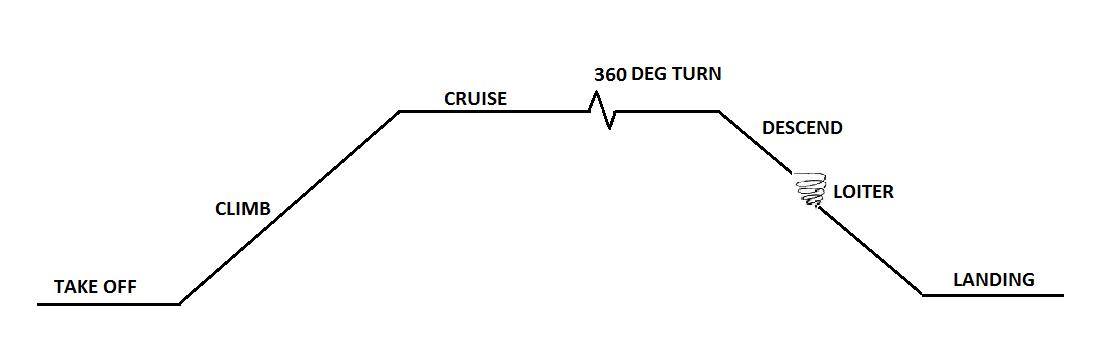
\includegraphics[width=4.5in]{figures/missionreq.jpg}
     \caption{Mission Profile}
       \label{fig:mission_profile}
    \end{center}
\end{figure}
%
\section{CONFIGURATION CHOICE}
Following are the salient features of the configuration considered:
\begin{itemize}
\item The airplane is a monoplane due to ease of construction and need for lesser
thrust to counter induced drag.
\item High wing of aspect ratio 8 was chosen because of stability considerations.
Also, most of the similar airplanes have a high wing configuration.
\item Airfoil was chosen to be S1223 because of its high lift characterestics, deep
camber and thin wing. It is also highly suitable for low speed flights
\item No wing sweep or taper was chosen due to ease of construction and the
fact that the airplane wing operates only in the low speed regime
\item A conventional tail was chosen as it provides adequate stability and control
and is easier to construct than other complex tail configurations
\end{itemize}
 
\section{SUMMARY OF WORK DONE AS PART OF THE AERODYNAMIC DESIGN}
%
Brief description accompanied by data/weight estimates and diagrams.
%
\subsection{Data Obtained from Literature Survey}
Table \ref{tab:lit_survey} gives the details of existing aircrafts of similar configurations for which data were accessible.
%
\begin{table}[H]
\begin{center}
\makebox[\textwidth]{
 \begin{tabular}{|c|c|c|c|c|}
 \hline
Parameters & Worchester & Worchester & Cincinnati & SAE MicroClass \\
 & I & Polytec. II & University & Entry\\
\hline
Gross Weight(kg) & 0.316 & 1.915 & 1.95 & 1.732\\
Payload Weight(kg) & 0.163 & 1.530 & 1.632 & 1.284 \\
Empty Weight(kg) & 0.153 & 0.384 & 0.316 & 0.448\\
Powerplant Weight(kg) & 85.4 & 0.185 & 0.3 & 0.368\\
Airfoil & S1223 & S1223 & S1223 & S1223\\
\hline
\end{tabular}}
\caption{Data of similar airplanes\cite{5}}
\label{tab:lit_survey}
\end{center}
\end{table}
%
\subsection{First Weight Estimate}
The first weight estimate of the aircraft was done based on data from our literature survey. The first weight estimate comes out to be 1.495 kg.
%
\subsection{Second Weight Estimate}
The second weight estimate was done by choosing our powerplant by taking data from the chosen airfoil. The chosen powerplant is 
\begin{itemize}
\item Motor : Avionic C3536 brushless motor (see \cite{1}) Prop : 11x7; 1.3 Kg thrust ; ESC 30A
\item Battery : 3S Lipo; 11.1V 25C, 2200 MaH (see \cite{2})
\end{itemize}
Taking into account the powerplant weight, the second weight estimate comes out to be 1.642 kg.
%
\subsection{Views of the Designed Airplane}
The three view configuration along with the 3D view is outlines in Fig \ref{fig:3view}
\begin{figure}[H]
\centering
\begin{minipage}{0.5\textwidth}
\begin{centering}
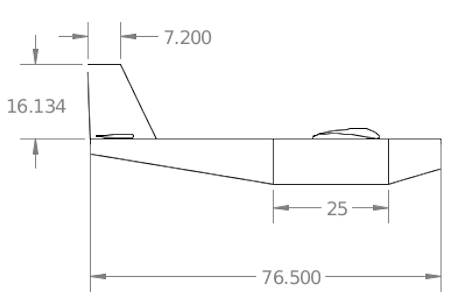
\includegraphics[width=\textwidth]{figures/side.png}
\centerline{\small (a) Side View}
\end{centering}
\end{minipage}
\hspace{2mm}
\begin{minipage}{0.4\textwidth}
\begin{centering}
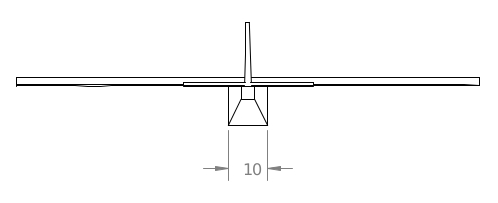
\includegraphics[width=\textwidth]{figures/front.png}
\centerline{\small (b) Front View}
\end{centering}
\end{minipage}
%
\vspace{0.1in}
\begin{minipage}{0.6\textwidth}
\begin{centering}
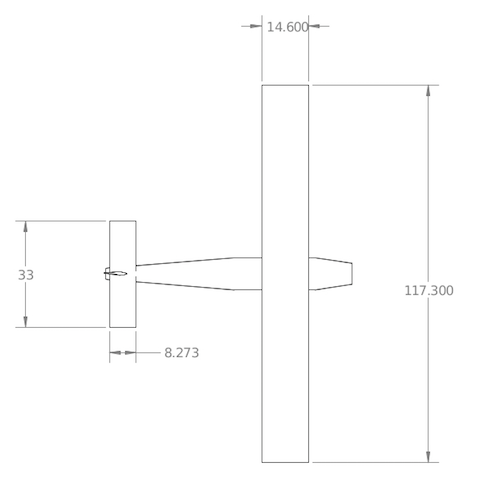
\includegraphics[width=\textwidth]{figures/top.png}
\centerline{\small (c) Top View}
\end{centering}
\end{minipage}
\hspace{2mm}
\begin{minipage}{0.4\textwidth}
\begin{centering}
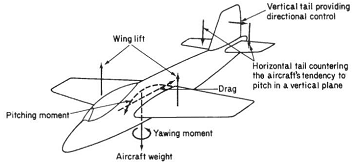
\includegraphics[width=\textwidth]{figures/3D.png}
\centerline{\small (d) 3D View}
\end{centering}
\end{minipage}
\caption{Three view and isometric view of the airplane}
\label{fig:3view}
\end{figure}
%
%
\subsection{V-n Diagram}
Figure \ref{fig:V_n_diag} shows the envelope of the final V-n diagram for the chosen aircraft.
%
\begin{figure}[H]
    \begin{center}
      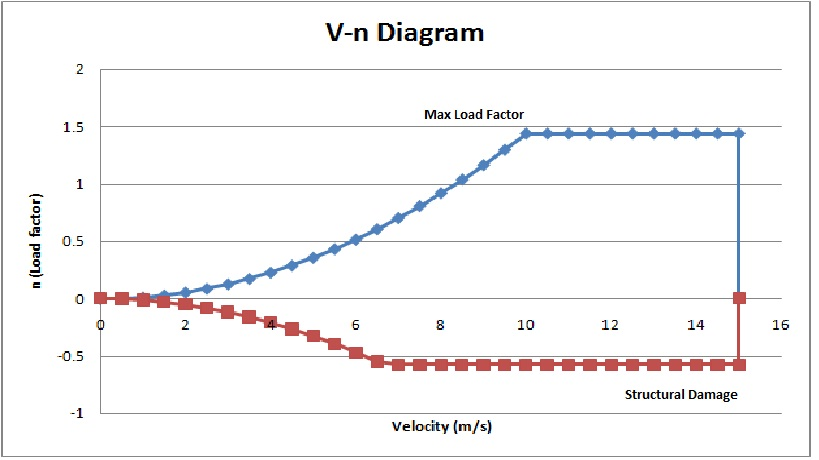
\includegraphics[width=6in]{figures/Vn_Dia.jpg}
\caption{Flight envelope: V-n diagram for the given airplane.}
       \label{fig:V_n_diag}
    \end{center}
\end{figure}
%
\subsection{Some performance parameters}
A few important performance parameters are highlighted below
\begin{enumerate}
\item Thrust-to-weight ratio : 0.63 (Considering 80\% efficiency)
\item Endurance : 4 min
\item Range : 2.4 km
\item Maximum Load Factor : 1.43
\item Take-off distance : 30 m
\item Landing distance : 50 m
\item Climb Angle : 6 deg
\item Wing Loading : 93.342 N/$m^2$
\end{enumerate}
%
\section{Bill of Materials with suggested Vendors}
Table~\ref{tab:bill_materials} gives the details of the materials required for fabrication as well as suggested vendors and approximate cost
\begin{table}[H]
\centering
\makebox[\textwidth]{
\begin{tabular}{|c|c|c|}
\hline
Component&Price(Rs)& Suggested Vendor \\
\hline
Motor & 1400 & See \cite{1}\\
Battery& 3395 & See \cite{2} \\
Balsa Wood& 4000 & \\
Aluminium & 1000 &  \\
ESC(electronic speed controller) & 1000 & See \cite{3} \\
Servo motors (4 Nos) & 1860 & See \cite{4}\\
Propeller 11x7 & 200 & RcBazaar \\
Miscellaneous & 2500 & \\
\hline
Total&15400& \\
\hline
\end{tabular}}
\caption{Aircraft cost estimation}
\label{tab:bill_materials}
\end{table}
%

% Shifted Biblography from here to the latest report.
%
